\documentclass[titlepage,11pt,twoside]{article}



\usepackage[dvips]{graphicx}

\usepackage[myheadings]{fullpage}
\usepackage{pmetrika}
\usepackage{pmbib}
\usepackage{color}
\usepackage{mathtools}
\usepackage{amssymb}
\usepackage{hyperref}
\usepackage{natbib}


%\usepackage{submit}

\newcommand{\bfU}{\mbox{\boldmath$\mathsf{U}$}}
\newcommand{\bfu}{\mbox{\boldmath$\mathsf{u}$}}
\newcommand{\hl}[1]{\textcolor{magenta}{#1}}
\newcommand{\RR}{\mathbb{R}}
\DeclareMathOperator*{\V}{V}
\newcommand{\argmax}{\text{argmax}}
\newcommand{\R}[1]{\texttt{#1}}
\newcommand{\acos}{\text{arccos}}


%\begin{figure}[h]
%\centerline{\includegraphics{figure03.eps}}
%\caption{Projection of item discrimination vectors onto $V_{\theta_T}$ hyperplance for a six item three-dimensional approximate sample structure.}
%\end{figure}


%\raggedbottom
\flushbottom


%\firstpage{1}
%\setcounter{lastpage}{999}
\setcounter{secnumdepth}{3}

\begin{document}

\linespacing{1}

%\title{Something that is not PCADSC}
%\title{Structure comparison for multivariate data by\ldots / with application to \ldots}
\title{Explorative data structure comparison with application to \ldots}

\author{Anne H. Petersen, Bo Markussen, Karl Bang Christensen}

\affil{University of Copenhagen}


\vspace{\fill}




\linespacing{1}

%\RepeatTitle{Psychometrics: From Practice to Theory and Back}

\begin{center}\vskip3pt


\vspace{32pt}

Abstract\vskip3pt

\end{center}


\begin{abstract}
abstract...
\begin{keywords}
keywords...
\end{keywords}
\end{abstract}

\vspace{\fill}\newpage

\section{Introduction}
\label{sec:introduction}

Classical statistical methodology is aimed at analyzing data from designed experiments and historically statistical analyses have been done by researchers who knew the design and origin story of the data set well. The origin stories of data sets have changed over time and today a lot of data is accumulated without specific purpose. This is due to vast amounts of data being registered online and to a trend towards more open source research. The latter phenomenon in particular poses new challenges wrt. data quality assessment. When data are collected and made public without a specific end-point in mind, how do we ensure that differences in, say, choice measurement instruments, mode of administration, or sampling frame do not cause the data to be effectively divided into subsets that are simply not comparable?

Surveys often use mixed modes of administration, e.g. mail and telephone, and while this can improve response rates, the mode of administration can affect results \cite{Brambilla1987,McHorney1994} and differences in response behavior can lead to biased results. Powers, Mishra and Young \citeyearpar{Powers2005} report effects of mode of administration on changes in mental health scores that are of a magnitude that is considered to be clinically meaningful.

The rapid growth of web surveys, due to low cost, timeliness, and other factors, generate large data sources that lack a sampling frame of the general population. However, it can be problematic to combine online panels (pre-recruited profiled pools of respondents) with intercept samples (a pool of respondents obtained through banners, ads, or promotions) \cite{Liu2016}.

Sophisticated methods for addressing this question are available when we are willing to assume a statistical model, but when these models are taken away, a remarkable void of methods is left behind. What is needed is a procedure that compares differences in overall data structures in two (or more) subsets of a dataset without assuming neither directional nor hierarchical relationships between the variables. We propose a new method for this task, namely Principal Component Analysis-based Data Structure Comparison (PCADSC). This method employs the principal component decomposition of the data matrix performed on two subsets of a dataset in order to create intuitive visualizations of data structure differences. \hl{Mention R package.}


This manuscript is structured as follows: First, in Section \ref{sec:stateoftheart}, we present the data structure comparison problem in more detail and discuss what statistical methods are already available for solving similar challenges. Next, in Section \ref{sec:pcadscintro}, we move on to a description of the PCADSC procedure, including a brief introduction to principal component analysis (PCA) in general. In Section \ref{sec:dataexample}, we present a worked data example using the open source, online available PISA data (\hl{ref}), which is an example of a dataset where multiple data collection methods \hl{Eller måske lande?} have been employed.




\section{Something about state of the art}
\label{sec:stateoftheart}
\subsection{\hl{More detailed description of the type of problem we wish to address}}
\hl{
\begin{itemize}
\item Two subsets of a dataset, i.e. to datasets with the same variables, but different observations
\item Wish to compare structures without specifying a model or even any variables of interest
\item The most central example is the question of whether the two subsets can readily be combined in a (unknown) data analysis, or if the subset-inducing variable actually implies heterogeneity across the subset division
	\begin{itemize}
		\item Examples: Large scale open source datasets such as the PISA data and ESS (European Social Survey) data and ...(?). In these datasets, the data producers are very far away from the majority of the data analysts. Therefore, problem-specific recommendations about potential instrument-induced challenges in the datasets are not available for the data analysts. How can data producers ensure that this will not be an issue, at least not related to known data gathering differences?
		\item Other examples?
		\item Perhaps a description of what happens if we are to combine the two subsets of the datasets without taking a e.g. an instrument-effect into account. When will it cause problems (maybe: causal graph style?)?
		\item Mention somewhere: We want a solution that is largely independent of the sizes of the two subsets of data. Thereby, a lot of methods that compare each subset to the full dataset in some sense are excluded.
	\end{itemize}	
\end{itemize}
}

\subsection{\hl{Describe existing methods used to solve similar questions or parts of the question we are addressing}}
\hl{
\begin{itemize}
\item The simplest case: variable-by-variable tests in distributional differences
	\begin{itemize}
		\item Simple, but scales poorly
		\item Only relates to marginal differences and not to the interplay between variables
	\end{itemize}
\item Karl's papers?
\item Anne's papers: IRT-based methods for surveys
	\begin{itemize}
		\item Moves beyond the marginal approach, but needs a model pre-specified
		\item Thus, it is not a general data structure comparison method, but rather a fitted-model comparison method. It addresses the interplay between the model and the data, not the data alone. This is fundamentally a different (though related) question.
	\end{itemize}
\end{itemize}
}


\section{PCADSC - description of the method}
\label{sec:pcadscintro}
\hl{Description from Anne's master's thesis. Rewrite.}

As mentioned above, the purpose of PCADSC is comparing overall data structures in two or more subsets of a dataset. But before we can get further into describing this procedure, we must first define what exactly is meant by "overall structure". One such definition is the structure of the covariance matrix of the dataset. If we assume all variables in the dataset to be jointly normal with zero means, the covariance matrix is a sufficient statistic for describing the simultaneous distribution of all the variables. This gives it a very nice interpretation as a measure of the overall structure. If we do not accept the normality assumption, pairwise correlations and variable variances are still interesting quantities that say something about the interrelations between the variables, at least in terms of linear relationships. All in all, the empirical covariance matrix is a reasonable place to start looking for differences in "overall data structures".

Though the idea sounds appealing, it is quite difficult to assess similarity of matrices, and moreover, this becomes increasingly difficult for large numbers of variables and thus high dimensional covariance matrices. There is simply too much information to consider at once.

However, by clever use of linear algebra, we can construct a decomposition of the covariance matrix that makes it easier to gain an overview of the data. We propose a new method based on principal component analysis that seems to be able to identify differences in datasets based on intuitive, visual inspections. We refer to this method as principal component analysis-based data structure comparison (PCADSC) and we present the procedure below. But first, we give a minimal introduction to principal component analysis in general with reference to Koch (2014).


\subsection{Principal component analysis}

Consider $n$ observations $x_1,\dotsc,x_n \in \RR^d$ of $d$ variables, let $\bar{x} = \frac{1}{n} \sum_{i=1}^n x_n$ denote their average and let $S = \frac{1}{n-1} \sum_{i=1}^n (x_i-\bar{x}) (x_i-\bar{x})^\top \in \RR^{d \times d}$ denote the empirical covariance. Suppose that we want to describe the observations by $q$ numbers instead of the original $d$ numbers. The associated \emph{rank-q-reconstruction error} is defined as the minimal squared error that is achievable by linear subspaces $K_q \subset \RR^d$ of dimension $q < d$, that is
\begin{equation*}
\min_{K_q} \sum_{i=1}^n \min_{z \in K_q} \lVert x_i - \bar{x} - z \rVert^2 =
\min_{K_q} \sum_{i=1}^n \lVert x_i - \bar{x} - \text{proj}_{K_q}(x_i - \bar{x}) \rVert^2.
\end{equation*}
\emph{Principal component analysis} (PCA) ensures the existence of a subspace $\hat{K}_q \subset \RR^d$ that attains this minimum, and it provides an explicit description of $\hat{K}_q$ and the rank-q-reconstruction error. Thus, let $S = U \Lambda U^\top$ be the eigenvalue decomposition of $S$. Here $\Lambda \in \RR^d$ is the diagonal matrix with the eigenvectors $\lambda_1 \ge \dotsm \ge \lambda_d \ge 0$ in the diagonal, and $U \in \RR^d$ is the orthogonal matrix with the associated eigenvectors $\eta_1,\dotsc,\eta_d \in \RR^d$ in the columns. The eigenvalues are uniquely defined, and the eigenvectors are uniquely defined up to a change of sign whenever the eigenvalues are different. If some of the eigenvalues are identical, e.g.\ $\lambda_i=\lambda_{i+1}=\dotsm=\lambda_j$, then the associated eigenvectors $\eta_i,\eta_{i+1},\dotsc,\eta_j$ are uniquely defined up to a common rotation. In practice this only happens if $n < d$, in which case the last $d-n$ eigenvalues will be zero. It is a result from linear algebra that the rank-q-reconstruction error for $q < d$ is achieved for
\begin{equation*}
\hat{K}_q = \text{span}\{\eta_1,\dotsc,\eta_q\}
\end{equation*}
and equals $\sum_{j=q+1}^d \lambda_j$. The eigenvectors $\eta_j \in \RR^d$ are called \emph{loadings}, and the eigenvalues $\lambda_j \ge 0$ may be understood as \emph{variation components}. The projections $\eta_j^\top (x_i - \bar{x})$ of the observations onto the loadings are called \emph{scores}. The $j$th loading can also found as the unit vector $u \in \RR^d$ orthogonal to $\hat{K}_{j-1}$, where the initial subspace is defined as $\hat{K}_0 = \{0\}$, that maximizes the variation of the associated scores
\begin{align*}
\eta_j &= \argmax_{u \in \RR^d\colon u \perp \hat{K}_{j-1}} \sum_{i=1}^n \lVert u^\top (x_i - \bar{x}) \rVert^2, &
\lambda_j &= \frac{1}{n-1} \sum_{i=1}^n \lVert \eta_j^\top (x_i - \bar{x}) \rVert^2.
\end{align*}
It is worth emphasizing that the greedy approach of successively adding the next direction $\eta_j$ explaining most of the remaining variation, also gives the sequence $\hat{K}_q = \hat{K}_{q-1} \oplus \text{span} \{\eta_q\}$ of subspaces minimizing the rank-q-reconstruction error. This strong interpretation of PCA, which is often overlooked in the literature, means that the sequence of loadings $\eta_j$ and their associated variation components $\lambda_j$ yield a simultaneous description of the structure of the data set for all approximating dimensions $q$. This implies that the loadings and variation components can be used to investigate the structure of the data set without the need to decide on an approximating dimension $q$.


%Principal component analysis (PCA) allows us to decompose a data matrix consisting of $n$ observations of $d$ variables into $d$ orthogonal vectors of length $d$. This is in itself not very impressive nor useful. But PCA does not result in just any basis of the data matrix. The basis chosen using PCA has the very favorable property that each vector is chosen such that they maximize the accumulated explained variance. These vectors are usually denoted \textit{principal component scores} or simply \textit{principal components} and they are constructed as linear combinations of the variables in the dataset (or, equivalently, as projections of the data matrix). The coefficients of each variable in these projections are denoted \textit{loadings}. Let $S \in \RR^{d \times d}$ denote the empirical covariance matrix and let $X \in \RR^{n \times d}$ denote our observed data matrix. $d$ is the number of variables while $n$ is the number of observations. The deconstruction procedure then goes as follows:
%\begin{enumerate}
%\item The vector of loadings corresponding to the first principal component, $\eta_1 \in \RR^d$, is chosen such that the component explains as much variance as possible. More precisely, for any unit vector $u \in \RR^d$ we find that $\V(u^T X^T)$ is maximized when $u = \eta_1$. Let $\lambda_1 = \V(\eta_1^T X^T)$.
%\item The second vector of loadings is then chosen as $\eta_2 = \argmax_{u: \, u \perp \eta_1} \V(u^T X^T)$ and we again define $\lambda_2 := \V(\eta_2 X)$.
%\item The third vector of loadings is $\eta_3 = \argmax_{u: \, u \perp \{\eta_1, \eta_2\}} \V(u^T X^T)$ and $\lambda_3 :=  \V(\eta_3^T X^T)$ \\
%\vdots
%\item[\refstepcounter{enumi} $d$.] The $d$th vector of loadings is $\eta_d = \argmax_{u: \, u \perp \{\eta_1, ..., \eta_{d-1}\}} \V(u^T X^T)$ and $\lambda_d = V(\eta_d^T X^T)$.
%\end{enumerate}
%The $\eta_i$s and $\lambda_i$s are determined uniquely (up to scaling) and they are given as the eigenvectors and eigenvalues of $S$, respectively. Moreover, we find that $X = \sum_{i=1}^d \eta_j \eta_j^T X$, so the procedure is really just a clever choice of rotation of the data, such that it is split up into vectors that are ordered by their variances, or more precisely, their variance contributions. We define the contribution to the total variance of the $k$th principal component as $\frac{\lambda_k}{tr(S)}$ and please note that, due to the properties of eigenvalue decomposition, $tr(S) = \sum_{i=1}^d \lambda_i$, which is the sum of the variances of the variables in the dataset.
%
% In this introduction, we have assumed full rank of the covariance matrix $S$ for simplicity, but it should be noted that this assumption is in no way needed for the results to hold.

\subsection{PCA-based data structure comparison}
Above, we promised a method for intuitive, visual inspection of data structure similarities, but as of now, all intuition might have been lost in technicalities. The main point we want to emphasize from PCA is that whereas the scores describe the observations, the variation components and the accompanying loadings describe the usage of the variables. If two different datasets with the same variables, but different samples of observations, have similar loading patterns, then the variables appear to be measuring the same underlying quantities in both data situations. This can be the case while the two sets of scores could be arbitrarily different, which e.g.\ could happen if the two datasets were taken from two different populations of subjects. On the other hand, if the loading patterns are different in the two datasets, then this indicates that the variables are used differently in the two data situations, and hence it would be criticizable to use these variables for comparisons across the two datasets.  

%Specifically, we can interpret the loadings as weights that determine the relative influence of each variable in each principal component.

%the two data sets will agree on which variables explain the most variance and also how this variance is explained.  Looking at the PCA loadings and the cumulative explained variance thus provides a straightforward non-parametric graphical approach for assessing similarity between two datasets.

In this paper we propose three diagnostic plots, referred to as the \emph{CumEigenPlot}, \emph{HairPlot} and \emph{PancakePlot}, for comparing the loading patterns in two datasets. In order to describe these plots we consider two different datasets in the same $d$ variables and with $n_1$ and $n_2$ observations, respectively. For dataset $i=1,2$ let $S_i \in \RR^{d \times d}$ be the empirical correlation matrix \hl{(find a way to introduce the empirial correlation matrix instead)}, and let $\lambda_{i1} \ge \dotsm \ge \lambda_{id} \ge 0 $ and $\eta_{i1},\dotsc,\eta_{id} \in \RR^{d}$ be the corresponding variation components and loadings. The correlation matrices correspond to the covariance matrices for the variables after these have been standardized to unit standard deviation separately within the two datasets. Similarly, let $S \in \RR^{d \times d}$ be the empirical correlation matrix for the combined dataset with $n_1+n_2$ observations, and let $\lambda_1 \ge \dotsm \ge \lambda_d \ge 0$ and $\eta_1,\dotsc,\eta_d \in \RR^d$ be the corresponding variation components and loadings.

\hl{To do: justification for using correlation matrices should be further elaborated. And also: Something about what to do if not all variables are numerical. Using correlation matrices is not the same as assuming standadized variables; there is a difference in the permutations.} 

\medskip

Description of the \emph{CumEigenPlot}: This plot compares the variation components. If these are the same in the two sample populations, then the best estimate for the variation components are $\lambda_1 \ge \dotsm \ge \lambda_d \ge 0$ found in the combined dataset. And we would expect $\lambda_{i1} \ge \dotsm \ge \lambda_{id} \ge 0$ for $i=1,2$ to be alike excepts sample variation. In order to investigate whether the same proportion of the total variation can be described by the same number of principal components in the two datasets we plot a piecewise linear curve connecting the points 
\begin{align*}
(0,0), &&
(\lambda_1,\lambda_{11}-\lambda_{12}), &&
(\lambda_1 + \lambda_2,\lambda_{11}+\lambda_{12}-\lambda_{12}-\lambda_{22}), &&
\ldots, &&
\bigg( \sum_{j=1}^d \lambda_j, \sum_{j=1}^d \lambda_{1j} - \sum_{j=1}^d \lambda_{2j} \bigg).
\end{align*}
This may be seen as a cumulated Bland-Altman plot for the variation components (\hl{reference to cumulated residuals and to Bland-Altman}). Note that since we are using correlation matrices the last point will always be $(d,0)$. Thus, this curve will begin and end at the x-axis. And the larger excursions it makes away from the x-axis the less alike the cumulated variation components for the two datasets are.

Whether the excursions in the observed curve are large or within the range of sample variation can be quantified by a permutation test. The idea is that we randomly reallocate the $n_1+n_2$ observations in the combined dataset to two datasets with $n_1$ and $n_2$ observations, respectively, and then repeat the procedure described above. The random reallocation by construction ensures that the two resampled datasets are alike except their sample size and sampling variation. In the \emph{CumEigenPlot} we make 1000 independent random reallocations, and plot the observed curve together with 20 of the resampled curves as well as a shaded region visualizing pointwise 95pct coverage intervals. This provides a graphical validation tool. P-values for the null hypothesis that the variation components are the same are easily provided for any appropriate test statistic by the resampling procedure as well. We have implemented the \emph{Kolmogorov-Smirnov} and the \emph{Cram\'er-von Mises} test statistics, which are given by
\begin{align*}
\text{KS} &= \max_{k=1,\dotsc,d} \bigg\lvert \sum_{j=1}^k \lambda_{1j} - \sum_{j=1}^k \lambda_{2j} \bigg\rvert, &
\text{CvM} &= \sum_{k=1}^{d-1} \frac{\lambda_k + \lambda_{k+1}}{2} \bigg( \sum_{j=1}^k \lambda_{1j} - \sum_{j=1}^k \lambda_{2j} \bigg)^2.
\end{align*}  

\medskip

Description of the \emph{HairPlot:} Let $\lambda_{\max} = \max\{ \lambda_{11}, \lambda_{21} \}$ be the largest variation component for the two datasets. The empirical correlation matrix $S_1$ for the first dataset has the following orthogonal decomposition in the coordinate system of the second dataset
\begin{equation*}
S_1 = \sum_{k=1}^d \lambda_{1j} \eta_{1k} \eta_{1k}^\top
= \lambda_{\max} \sum_{k=1}^d
\Bigg( \sum_{j=1}^d \sqrt{\frac{\lambda_{1k}}{\lambda_{\max}}} (\eta_{1k} \eta_{2j}^\top) \eta_{2j} \Bigg)
\Bigg( \sum_{j=1}^d \sqrt{\frac{\lambda_{1k}}{\lambda_{\max}}} (\eta_{1k} \eta_{2j}^\top) \eta_{2j} \Bigg)^\top,
\end{equation*}
and we have a similar decomposition of $S_2$ in the coordinate system of the first dataset. We propose to visualize these two decompositions in a $d \times d$ grid display. In the $j$th row and $k$th column of this display we plot two arrows based at the lower left corner of the grid cell. The first arrow has length $\mu_{jk}$ and angle $\theta_{jk}/2$ anticlockwise from the diagonal, and the second arrow has length $\nu_{jk}$ and angle $\theta_{jk}/2$ clockwise from the diagonal. To facilitate the following description we will refer to the arrows drawn anticlockwise as the blue arrows, and the arrows drawn clockwise as the red arrows. The lengths $\mu_{jk}$ and $\nu_{jk}$ and the angle $\theta_{kj}$ are given by
\begin{align*}
\mu_{jk} &= \sqrt{\frac{\lambda_{1k}}{\lambda_{\max}}} \lvert \eta_{1k} \eta_{2j}^\top \rvert, &
\nu_{jk} &= \sqrt{\frac{\lambda_{2j}}{\lambda_{\max}}} \lvert \eta_{2j} \eta_{1k}^\top \rvert, &
\theta_{jk} &= \acos(\lvert \eta_{1k} \eta_{2j}^\top \rvert).
\end{align*}

The absolute value of the projection $\eta_{1k} \eta_{2j}^\top$ is inserted due to the indeterminacy of the direction of loading vectors. This indeterminacy implies that the angle between loadings from the two datasets always can be chosen to be in the interval $[0,\pi/2]$, and hence the decomposition of $S_1$ and $S_2$ can be visualized in a joint plot by dividing the angles by two and using anticlockwise and clockwise shifts from the diagonal. Furthermore, the scaling of the lengths by $\lambda_{\max}$ is made so that the longest arrow has at most unit length.

In the \emph{HairPlot} the blue arrows in the $k$th column of the grid display visualize the decomposition of the $k$th principal components for the first dataset in the coordinate system of the second dataset. Similarly, the red arrows in the $j$th row visualize the decomposition of the $j$th principal components for the second dataset in the coordinate system of the first dataset. If the structures of the two datasets are identical, then we will have coinciding blue and red arrows along the diagonal in the grid display, and nothing else as arrows in the off-diagonal cells would have zero length. Differences in the variation components are visualized as differences in the lengths of the blue and the red arrows, also in the diagonal. And loadings in other directions than the corresponding loading from the other dataset are visualized as angle separation of the blue and the red arrows in the diagonal cells as well as arrows of non vanishing length in the off-diagonal cells.

%Using the same grid display, but interchanging the first and the second dataset as well as the rows and the columns, and using the angles clockwise, similar arrows are plotted in a different color.

%In our implementation we have used blue for the first and the second set of arrows, respectively.

\bigskip

Remarks: Presently permutation tests based on the Kolmogorov-Smirnov and the Cram\'er-von Mises test statistics has been implemented for CumVarAgreement. This should also be possible for the Hairplot based on the off-diagonal components. For the Pancakeplot a Wallyplot has been implemented (however, in Claus' Wally plot the position of the ``observed dataset'' is also random).

\bigskip

Description of the \emph{PancakePlot}: Our proposal of a PCADSC method consist of three steps. These steps should be performed separately for each of the two (or more) datasets that we wish to compare. Note that the datasets must have the same variables, but different sample sizes are allowed. The three steps are:
\begin{enumerate}
\item \hl{Standardize. Full data or subsets? And also: Something about what to do if not all variables are numerical.}
\item Compute the PCA loadings and the variance contributions of each principal component.
\item For each principal component, standardize the loadings, i.e. scale them such that they sum to one.
\item Produce a plot consisting of a bar for each principal component, decorated with the cumulative variance contribution corresponding to this component. The bar should be of length one and colored according to the variables loading the component.
\end{enumerate}
The plots resulting from this procedure should be inspected focusing on two properties: Similarities in loading patterns, which will correspond to similar visual impressions, and similarities in variance contributions.  \hl{Refer to example/show plot.}




\section{Data example stuff}
\label{sec:dataexample}
We will now turn to a concrete data example in order to illustrate the possibilities of each of the methods presented above \hl{more than just PCADSC?}. We use data from the 2012 version of the European Social Survey (ESS) project, a very large dataset that is freely available online at \url{www.europeansocialsurvey.org}. As the name suggests, the data comes from a survey that was conducted primarily in Europe aiming to collect information about the social conditions of the citizens \hl{reference?}. As with all international (or, simply, multi-center) studies, one might be concerned about whether or not the data from different countries can readily be combined. This is the question we will address using PCADSC in the current section.

All computations and figures presented in this section where created using our \R{R} package \R{PCADSC}, which is available online at \url{www.github.com/AnnePetersen1/PCADSC} \hl{maybe do a CRAN submission instead?}.

\subsection{Data}
\begin{figure}
\center
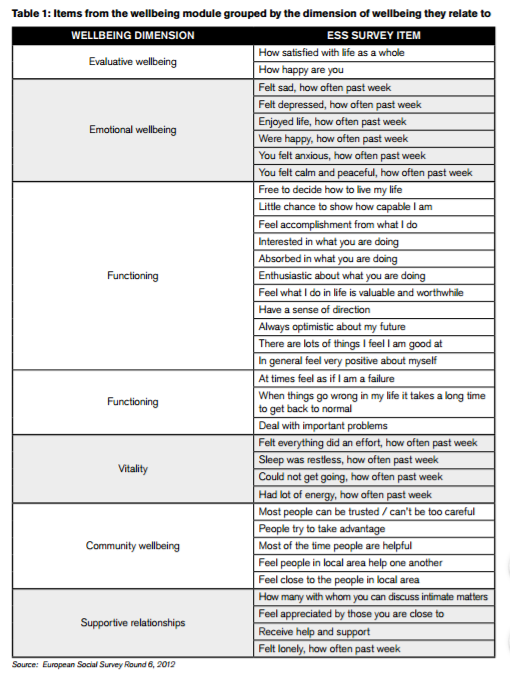
\includegraphics[scale=1]{surveyTable.png}
\caption{\hl{Make a new table here}}
\label{surveyTable}
\end{figure}
The ESS 2012 data contains a total of 626 variables collected from 54673 citizens in 29 countries. Here, we will only work with a subset of 35 questionnaire items that are all related to psychological well-being. These 35 items can be divided into 6 distinct scales (\hl{REF: ESS6 Topline Results Series 5}), as illustrated in Figure \ref{surveyTable}. We represent each of these scales by a single variable, which is calculated as the average score within the items related to that variable (\hl{ref to someone that says that is sensible?}). For simplicity, we use only complete cases for this construction and thus exclude all participants that did not answer all the 35 questionnaire items used below.

In the following, we only compare two countries, namely Denmark and Bulgaria, which have $n_{BG} = 1798$ and $n_{DK} = 1498$ complete cases in the variables of interest, respectively. For these two countries, the ESS authors \hl{different term?} particularly highlight differences in the relationship between the psychological well-being scales, at least on an nation-aggregated level (\hl{REF: ESS6 Topline Results Series 5}). This might be the result of large, cultural and socio-economic differences between the two countries. Simply put, we do not expect happiness and psychological well-being to be the same phenomena in Bulgaria and Denmark \hl{more here about why, about the cultures?}. Therefore, a successful method for data comparisons should be able to detect these differences by looking at the differences in the interplay between the 6 scales of psychological well-being.

\subsection{PCADSC}
\begin{figure}
\center
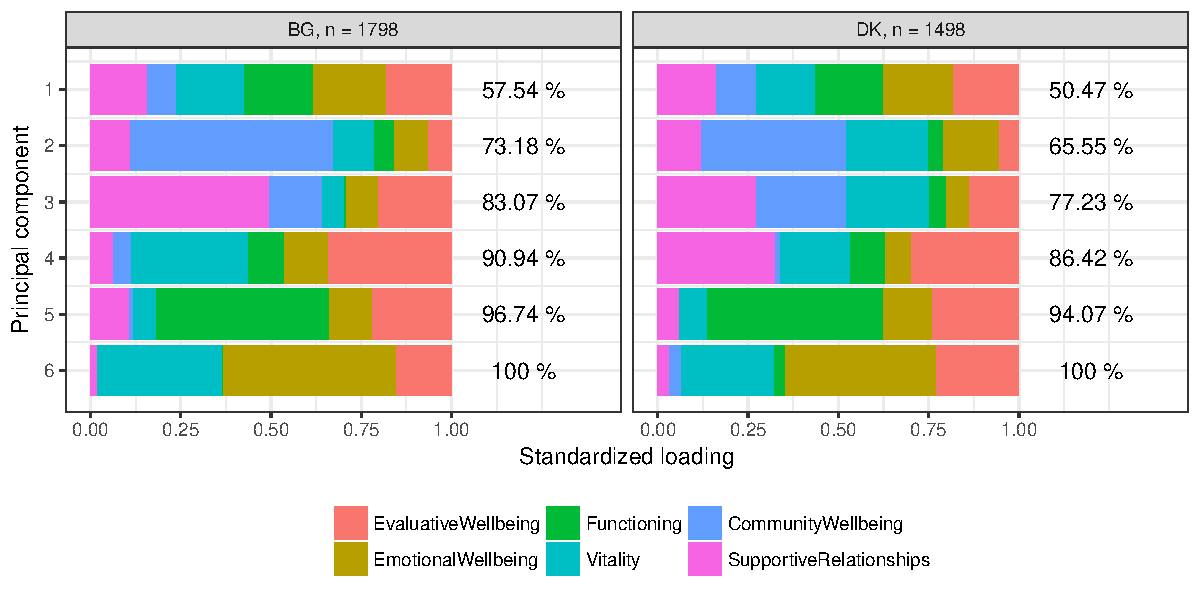
\includegraphics[scale = 0.8]{essPCADSC.pdf}
\caption{\hl{something}}
\label{plotESSPCADSC}
\end{figure}

\begin{figure}
\center
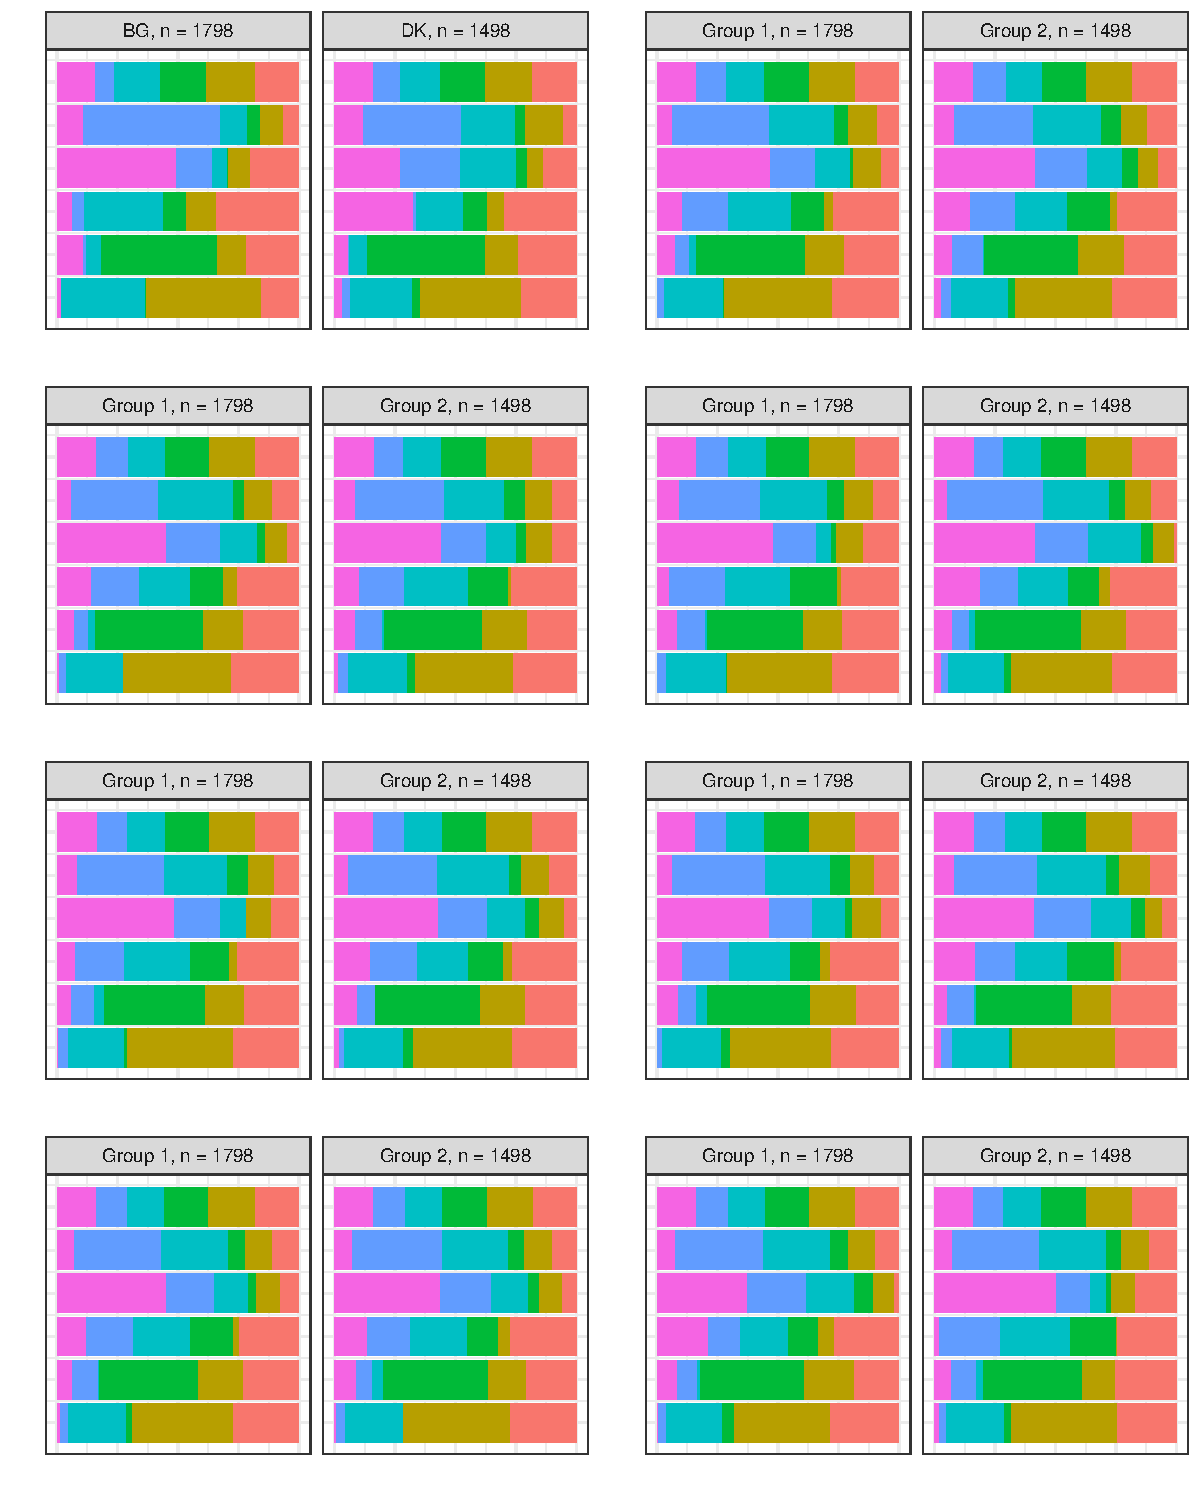
\includegraphics[scale = 0.8]{essWallyPCADSC.pdf}
\caption{\hl{something.}}
\label{plotESSPCADSCWally}
\end{figure}

\begin{figure}
\center
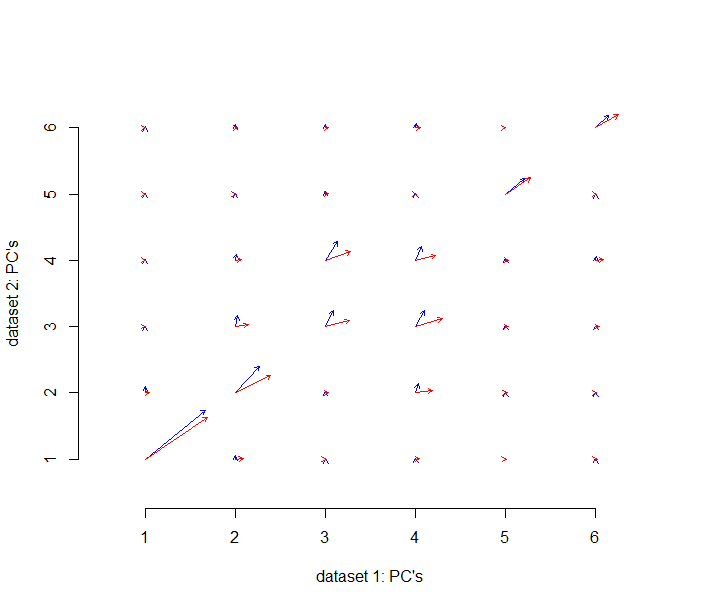
\includegraphics[scale = 0.8]{essHairplot.png}
\caption{The blue arrows show the principal components of the first dataset decomposed in the coordinate system of the principal components of the second dataset. And the red arrows the reverse.}
\label{plotESSHairplot}
\end{figure}

\begin{figure}
\center
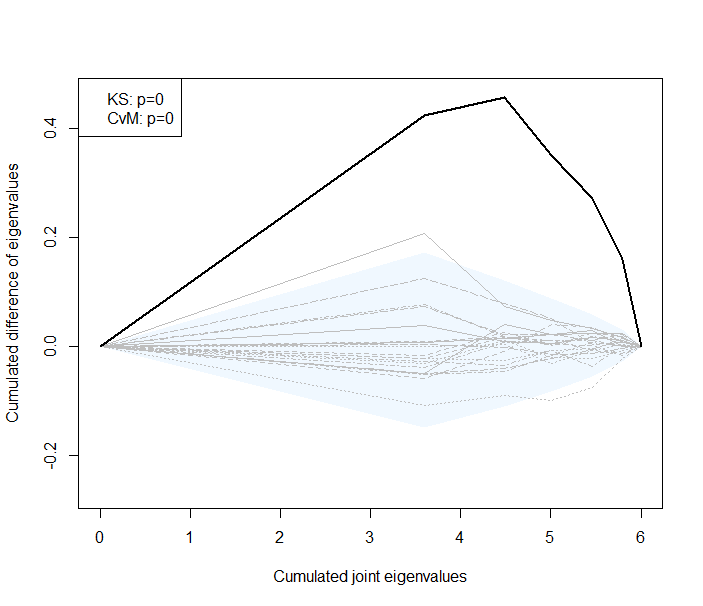
\includegraphics[scale = 0.8]{essCumVarAgreement.png}
\caption{\hl{something.}}
\label{plotCumVarAgreement}
\end{figure}

Figure \ref{plotESSPCADSC} illustrates the results of conducting PCADSC on the psychological well-being data from the ESS. While the first principal component, which is responsible for explaining 50-60 \% of the variance in the data, is very similar for the two countries, we see quite large differences in the remaining components. In the second component, we see that the two countries disagree in the relative importance of the scales \textit{Community wellbeing} and \textit{Vitality}. In the third and fourth components, general disagreement  is found. All in all, components 2-4, representing almost half of the variability in the data, are not very similar across the two countries. Moreover, the two subsets of the data also differ with respect to how much variance is explained by each component, and the difference is particularly big for the first component. This component has approximately 15 \%  more explanatory power in the Bulgarian subsample than it does in the Danish.

{\color{red}
Figure \ref{plotESSHairplot} shows the hairplot. The blue arrows visualize the decomposition of the principal components for the first dataset in the coordinate system of the second dataset. We see that PC2 also loads on PC3, that PC3 also loads on PC4, and that PC4 also loads on PC2 and PC3. The red arrows visualize the decomposition of the principal components for the second dataset in the coordinate system of the first dataset. We see that PC2 also loads on PC4, that PC3 also loads on PC2 and PC4, and that PC4 also loads on PC3. For PC1, PC5 and PC6 the main difference is in the size of the variation component.
}


In summary, we find that the datasets are fundamentally different and that we should therefore be wary about combining them in a joint analysis, which was also the conclusion of the ESS authors, though based on country-level aggregated statistics. \\


But did we really illustrate a data structure difference due to country differences or did we just illustrate the variability of the results of the PCADSC method? In order to investigate this further, we look at a so-called \textit{Wally plot} (\hl{ref: Claus Ekstrøm}). In this plot, we compare the results of PCADSC conducted with grouping by country with several random, but similar grouping variables. Specifically, we produce 7 PCADSC plots where the country variable was replaced by a randomly generated variable that divides the observations into two groups of the same sizes as the country samples. The results are illustrated in Figure \ref{plotESSPCADSCWally}. Here, we see that the differences in the second component from the original PCADSC results are not matched in any of the randomly grouped PCADSC runs. In fact, the 7 runs are remarkably similar, thereby illustrating that PCADSC seems to be very robust with respect to random groupings: The signal in the data is not blurred by the random subdivisions. When it comes to the differences in the third component for the two groups, we find much larger variability in the 7 random runs. \hl{more comments here... Wait until we are sure exactly what we think about the results and what other PCA-based methods, we will do before/after. Particularly, how do we deal with eigen value differences?}



\section{Discussion}
\label{sec:discussion}
\hl{
\begin{itemize}
\item Generalizing the results to non-numeric variables?
\item Generalizing the results to covariance matrices that are not of full rank?
\item ?
\end{itemize}
}

\section{Concluding Remarks}
\label{sec:conclusion}

\vspace{\fill}\clearpage
\newpage
\bibliographystyle{apa}
\bibliography{bib}

\end{document}
